\documentclass[12pt, a4paper]{article} %,twoside

\usepackage[literat, microtype, nocolor]{derradeiro}


\setcounter{secnumdepth}{0}

\begin{document}


В результате недавних археологических исследований на острове Paxos оказалось, что существовавший парламент функционировал вопреки приверженности законодателей к странствованиям. Копии записей парламента, хранимые каждым законодателем, были согласованы, несмотря на их частые уходы по важным делам и забывчивость посыльных. Протокол парламента жителей Paxos описывает новый подход к реализации автоматов в распределённой системе.

Представленное было обнаружено недавно за систематизацией материалов в офисе редакции TOCS. Несмотря на древность, главный редактор считал что материал не стоит публикации. Так как автор был занят работой на греческих островах, меня попросили подготовить этот материал.

Автором работы был археолог, который лишь немного интересовался компьютерными науками. К сожалению; ведь даже при условии, что цивилизация Paxon была мало изучена и непонятна, как описывает автор, их законодательная система --- это исключительный пример того, как можно реализовать распределённую систему, работающую в асинхронной среде. Действительно, набор усовершенствований добавленных жителями Paxon в свой протокол оказались не известными в технической литературе.

Автор даёт краткое описание связи Парламента цивилизации Paxon и распределённых вычислений в секции 4. Информатики возможно захотят прочитать эту секцию в первую очередь. И даже раньше они могут обратиться к объяснению алгоритма для информатиков автора Lampson[1996]. Более формально алгоритм описан De Prisco [1997]. Я также добавил дополнительные комментарии о относимости древнего протокола и более современных разработок в конце четвертой секции.

\newpage
\section{Проблема}
\subsection{Остров Paxos}

В начале тысячелетия, эгейский остров Paxos был процветающим торговым центром. Богатство привело к политическому совершенству, и паксоны заменили древнюю теократию парламентской формой правления. Однако торговля всё же стояла на первом месте по отношению к политической ответственности и ни один паксон не горел желанием посвятить свою жизнь парламенту. Парламент должен был функционировать даже при условии, что законодатели постоянно то уходили, то приходили в законодательную палату.

Проблема управления парламентом с частичной занятостью оказывается удивительно схожей с актуальной проблемой создания отказоустойчивых распределённых систем, где законодатели соответствуют процессам, а покидание парламента --- ошибке при обработке. Решение паксонов может заинтересовать информатиков. Я представляю небольшой исторический рассказ о протоколе парламента Paxon, продолжаемый ещё более коротким описанием его отношения к распределённым системам.

Цивилизация Paxon была уничтожена иностранным вторжением, и только недавно археологи начали раскапывать их историю. Наши знания об их парламенте в силу этих обстоятельств достаточно фрагментарны. Несмотря на то, что базовый протокол известен, мы очень плохо осведомлены о многих деталях. Тогда как именно эти детали представляют наибольший интерес. Я возьму ответственность за предположения о том, что же в действительности совершили паксоны.

\subsection{Требования}

Главной задачей парламента заключалась в определении закона (земли), определяемого последовательностью принятых декретов. В современном парламенте бы наняли секретаря для их записи, но среди паксонов не было желающих выполнять эту роль на протяжении всего заседания. Вместо этого, каждый законодатель хранил книгу учёта в которой и делал нумерованные записи принятых декретов. Например, в книге законодателя $\Lambda\iota\nu\chi\partial$ находилась запись:
\[
    155: \textup{Налог на оливки составляет 4 драхмы за тонну}
\]
если они считала, что 155 декрет парламента был принят и устанавливал размер налога на тонну оливок в 3 драхмы. Законодатели писали несмываемыми чернилами так что записи нельзя было изменить. 

Первое требование протокола парламента заключалось в корректности записей в учётных книгах, означающей, что не в каких двух книгах не могло быть противоречивой информации. Если законодатель $\Phi\iota\partial\epsilon\rho$ хранил в своей книге запись 
\[
    132: \textup{Лампы должны использовать только оливковое масло}
\]
то никто другой не мог хранить другую запись для декрета с номером 132. Однако другие законодатели могли под этим номером записи не иметь, если он не знал был ли такой декрет принят.

Соответствие книг учёта было недостаточным, так как они могли быть попросту все пустыми. Должно было быть такое требование, которое бы гарантировало, что декреты в конце концов всё-таки были бы приняты и записаны в книги. В современном парламенте, препятствием к принятию декрета могло быть несогласие среди законодателей. Но такого не было среди паксонов, среди которых преобладала атмосфера взаимного доверия. Законодатели паксонов имели желание принять каждый декрет, выносимый на рассмотрение. Но странствующий уклад жизни был проблемой. Корректность была бы потеряна, если бы одна группа законодателей приняла декрет 
\[ 
    37: \textup{Рисовать на стенах храма запрещено}
\]
а потом ушла на банкет, в то время как другая группа посетила зал заседания и, не зная ничего о том, что произошло, приняла противоречащий закон 
\[
    37: \textup{Свобода художественного самовыражения гарантирована} 
\]

Прогресс не мог быть гарантирован, пока достаточное число законодателей не оставалось в палате достаточное количество времени. Потому как законодатели паксонов не хотели сокращать свои дела не связанные с парламентом, быть уверенным, что когда-нибудь будет принят какой-либо декрет было невозможно. Однако, законодатели желали гарантировать, что находясь в палате, они и их помощники будут действовать без промедлений по всем вопросам парламента. Эта гарантия позволяла вывести протокол парламента, удовлетворяющий следующему условию прогресса:

    Если большинство законодателей\footnote{dd} находились в палате и никто не покидал или входил в палату в течении достаточно долгого периода времени, тогда любой декрет, вынесенный на рассмотрение будет принят и окажется записан во все книги учёта всех законодателей в палате.

\subsection{Допущения}

Требования протокола парламента могли быть удовлетворены только при обеспечении законодателей всеми необходимыми ресурсами. Каждый законодатель получал здоровую книгу для записи декретов, ручку и запас несмываемых чернил. Законодатели могли забывать что они делали после ухода из палаты, поэтому они делали записи о важных задачах в конце книги. Строку в списке декретов нельзя было изменить, но записи в конце можно было (спокойно) вычеркнуть. Для достижения условия прогресса необходимо было, чтобы законодатели могли измерять количество прошедшего времени, и для этого им выдавались простые песочные часы.

Законодатели таскали свои книги всё время и могли всегда прочитать список декретов и любую незачёркнутую запись. Листы книги были изготовлены из тончайшего пергамента, поэтому использовались для самых важных записей. Законодатель мог записать менее важные вещи на листке бумаги, который он мог (или не мог) потерять, когда уходил из парламента.

С той акустикой зала, которая была в палате ораторствовать было совершенно невозможно. Заседающие могли общаться только через посыльных и были снабжены достаточным количеством денег для найма такого их количества, которое им было нужно. Посыльный должен был учесть, что не может исказить сообщение, но ему позволялось забыть, что он только что доставил сообщение и передать его заново. Как и законодатели, посыльные посвящали работе в парламенте только часть времени. Посыльный мог покинуть палату по важному делу, например шестимесячное путешествие, прежде чем доставить сообщение. Он мог также больше никогда не возвращаться, что таким образом делало сообщение потерянным.

Хотя законодатели и посыльные могли приходить и уходить в любое время, в пределах палаты они посвящали всё работе связанной с парламентом. Многие специалисты не принимают эту информацию серьёзно, считая её пропагандой, чтобы изобразить Paxos как землю с более высокими моральными ценностями, чем соседи на востоке. Нечестность, хоть и редко, конечно же была. Однако, в силу того, что ни в одном официальном документе об этом не упоминается, мы имеем слабое представление о то, как они справлялись с нечестным поведением законодателей и посыльных. В секции 3.3.5 будет описаны факты, к которым мы пришли, в проблема.

\section{Синод одного декрета}

Парламент Paxon эволюционировал из раннего церемониального Синода жрецов, который собирался каждые 19 лет для выбора единого, воплощенного в записи декрета. На протяжении многих веков Синод выбирал декрет процедурой взаимного соглашения, требующей присутствия всех членов (жрецов). Но по мере процветания торговли, жрецы стали уходить и приходить в палату как придётся в то время как шло заседание. В конце концов, старый порядок (протокол) перестал работать и заседание окончилось не приняв декрета. Чтобы предотвратить повторения теологической катастрофы, лидеры цивилизации паксон обратились к математикам, чтобы они сформулировали протокол выбора декрета Синода. Требования и допущения протокола были по существу такими же, какие использовались в потом в парламенте, за исключением того, что книга содержала 1 декрет вместо многих. Завершённый протокол Синода описан далее, а протокол парламента в секции 3.

Математики выводили протокол Синода в несколько шагов. Во-первых, они доказали, что протокол, удовлетворяющий набору ограничений будет гарантировать согласованность  и прогресс. \textit{Предварительный протокол} был выведен следом из этого набора ограничений. Ограниченная  версия предварительного протокола,\textit{базовый протокол}\footnote{basic protocol}, гарантировала согласованность, но не прогресс. Завершённый протокол Синода, удовлетворяющий требованиям согласованности и прогресса был получен из базового ввода дополнительных ограничений\footnote{
    Подробная история создания протокола Синода не известна. Как современные информатики, математики паксонов описывали элегантные, логические выводы, которые не имели ничего общего с тем, как выводят алгоритмы. Однако, известно, что результаты математиков (Теорема 1 и 2 из секции 2.1) действительно предшествовали протоколу. Они были выведены, когда математики, в ответ на запрос создания протокола, пытались доказать, что такого протокола не существует.
}.

\subsection{Результаты математиков}

Декрет Синода выбирался серией пронумерованных \textit{бюллетеней}, где бюллетень был результатом референдума одного декрета. В каждом бюллетене, жрец мог только либо проголосовать за декрет или не проигнорировать его\footnote{Как и некоторые современные нации, Paxos не полностью понимали природу Афинской демократии.}. Набор жрецов, называемых \textit{кворумом} ассоциировался с каждым бюллетенем. Бюллетень считался успешным тогда и только тогда, когда каждый жрец в кворуме проголосовал за декрет.  Формально, бюллетень $B$ состоял из 4-х компонентов. (Пока не сказано обратно, \textit{набор} обозначает \textit{конечный набор}\footnote{Несмотря на то, что математики Paxon были очень развитым для того времени, они очевидно не имели знаний о теории множеств. Я взял на себя ответственность в переводе более примитивной нотации в язык современной теории множеств}.)
\begin{table}[h]
\begin{tabular}{ll}
    $B_{dec}$ & Декрет (тот, за который проголосовали)\\
    $B_{qrm}$ & Непустой набор жрецов (кворум бюллетеня)\\
    $B_{vot}$ & Набор жрецов (тех, которые голосуют за декрет)\footnote{Только жрецы кворму действительно голосовали, но математики Paxon выяснили, что будет проще убедить людей, что протокол верен, если в их доказательстве они позволят голосовать любому жрецу за любой бюллетень.}\\
    $B_{bal}$ & Номер бюллетеня
\end{tabular}
\end{table}

Бюллетень $B$ называелся \textit{успешным} титтк $B_{qrm} \subseteq B_{vot}$ так, что успешный бюллетень соответствует тому, за который проголосовали все члены кворума.

Номера бюллетеней выбирались из бесконечного упорядоченного набора чисел. Если $B_{bal}' > B_{bal}$, тогда бюллетень $B'$ назвался более поздним, чем $B$. Однако, это никак не отражало тот порядок, в котором бюллетени обрабатывались; более поздний бюллетень мог быть обработан перед ранним.

Математики Paxon определили 3 ограничения над набором $\mathcal{B}$ бюллетеней и далее показали, что обеспечивается согласованность, а прогресс может иметь место, если обрабатываемый набор бюллетеней соответствовал этим ограничениям. Первые два ограничения были простыми; они могут быть сформулированы неформально следующим образом.
\begin{table}[h]
\begin{tabular}{ll}
    $B1(\mathcal{B})$ & Каждый бюллетень в \mathcal{B} обладает уникальным номером.\\
    $B2(\mathcal{B})$ & Кворумы любых двух бюллетеней в \mathcal{B} включают хотя бы одного общего жреца.
\end{tabular}
\end{table}

Третье ограничение было более сложным. Один манускрипт Paxon содержал следующее, достаточно запутанное утверждение.
\begin{table}[h]
\begin{tabular}{ll}
    $B3(\mathcal{B})$ & Для каждого бюллетеня $B$ в $\mathcal{B}$, если любой жрец в кворуме голосовал за \textit{предыдущий} бюллетень в $\mathcal{B}$, тогда декрет $B$ эквивалентен декрету последнего бюллетеня из ранних бюллетеней. 
\end{tabular}
\end{table}

Интерпритация этого загадочного текста облегчалась манускриптов, изображённым на рисунке 1, который иллюстрирует условие $B3(\mathcal{B})$ с набором $\mathcal{B}$ из пяти бюллетеней для Синода, состоящего из пяти жрецов $\Alpha$, $\Beta$, $\Gamma$, $\Delta$ и $\Epsilon$. Этот набор $\mathcal{B}$ состоящий из пяти бюллетеней, где для каждого бюллетеня, набор голосующих --- подмножество жрецов кворума, чьи имена заключены в рамки. Например, номер бюллетеня 14 содержал декрет $\alpha$, кворум, состоящий из трёх жрецов и набор из двух голосующих. Условие $B3(\mathcal{B})$ имело вид "для каждого $B$ в $\mathcal{B}$: $\ldots$", где "$\ldots$" --- это условие бюллетеня $B$. Условия пяти бюллетеней $B$ Рисунка 1 следующие.

%\begin{figure}[h]
% \centering
%    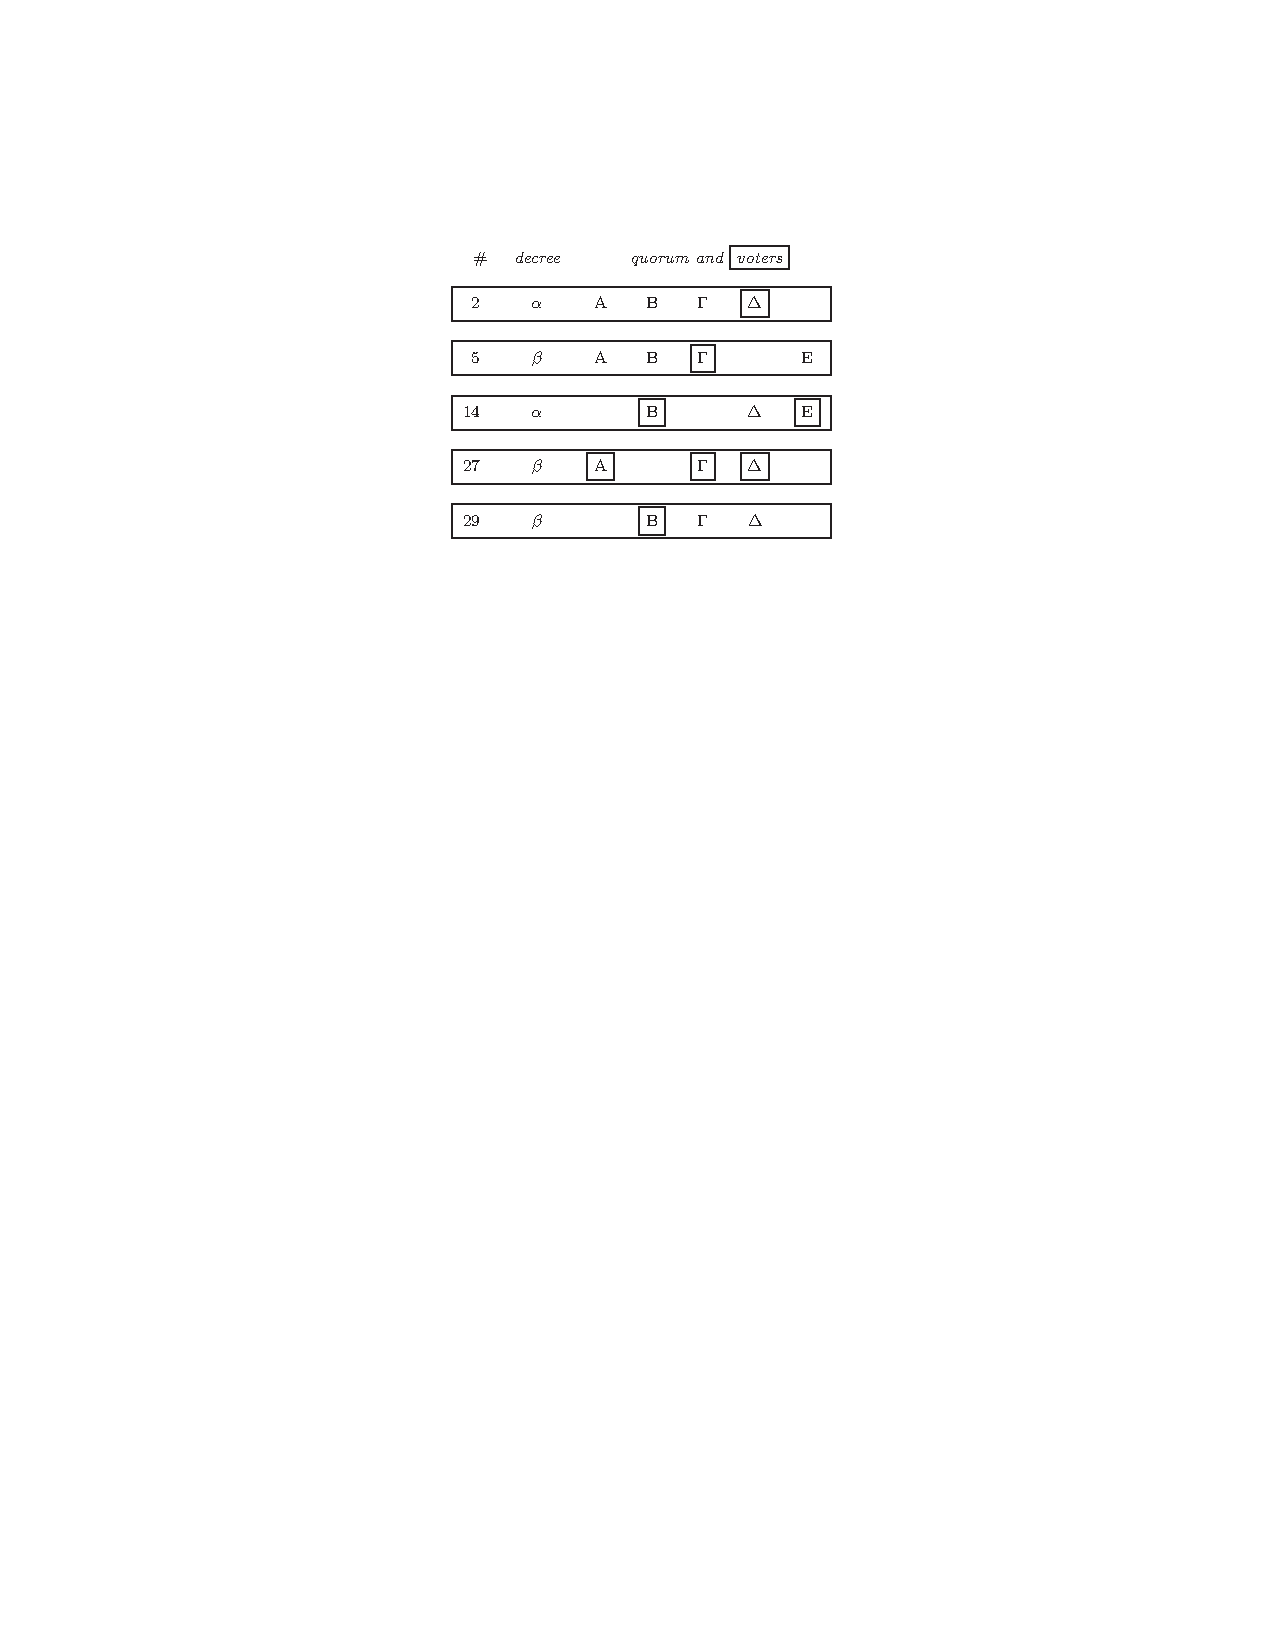
\includegraphics[width=0.6\textwidth]{images/Paxon-manuscript.pdf}
%\end{figure}

\begin{itemize}
    \item[2.] Бюллетень с номером 2 --- самый ранний бюллетень, поэтому его ограничение тривиальное и равно истине
    \item[5.] Ни один из членов кворума бюллетеня под номером 5 не голосовал за ранний, так что ограничение также просто равное истине
    \item[14.] Единственный член бюллетеня 14, который голосовал за предыдущие это $\Delta$, проголосовавший за номер 2, так что условие требует того, чтобы декрет 14 бюллетеня был также декретом 2-ого.
    \item[27.] (Успешный бюллетень.) Члены кворума 27-ого бюллетеня: $\Alpha$, $\Gamma$ и $\Delta$. Жрец $\Alpha$ не голосовал за ранние бюллетени, единственный ранний бюллетень за который голосовал $\Gamma$ это 5-ый, а $\Delta$ оставил голос за 2. Последний из этих двух бюллетений --- пятый, таким образом согласно ограничению декрет 27-ого бюллетеня должен совпадать с 5-ым.
    \item[29.] Члены кворума бюллетеня 29: $\Beta$, $\Gamma$ и $\Delta$. $\Beta$ уже один раз проголосовал за 14, жрец $\Gamma$ за 5 и 27, а $\Delta$ голосовал за 2-й и 27-й. Самый поздний из четырёх бюллетений --- 27, поэтому условие требует, чтобы 29 декрет совпадал с 27.
\end{itemize}


Чтобы утверждать $B1(\mathcal{B})$ --- $B3(\mathcal{B})$ формально требуется дополнительная нотация (определения). \textit{Голос} $v$ был определён как элемент, состоящий из трёх компонетов: жреца $v_{pst}$, бюллетеня $v_{bal}$ и декрета $v_{dec}$. Он представляет голос осуществлённый жрецом $v_{pst}$ за декрет $v_{dec}$ в бюллетене $v_{bal}$. Паксоны также ввели $null$ голоса, такие, что $v_{bal}=-\infty$ и $v_{dec}=\mathsc{BLANK}$, где $-\infty < b < \infty$ для любого номера бюллетеня $b$ и $\mathsc{BLANK}$ не являющийся декретом. Для любого жреца $p$, они ввели $null_p$ как уникальный голос $v$, где $v_{pst}=p$.

Математики Paxon определили полное упорядочение над множеством всех голосов, но часть манускрипта, содержащая эту информацию была утеряна. Сохранившийся фрагмент подсказывает, что для любого голоса $v$ и $v'$, при условии, что $v_{bal} < v_{bal}'$ выполняется $v < v'$. Нет информации о том, в каком порядке идут $v$ и $v'$, если $v_{bal} = v_{bal}'$.

Для любого множества $\mathcal{B}$, множество $Votes(\mathcal{B})$ голосов в $\mathcal{B}$ было определено состоящим из голосов $v$, таких, что $v_{pst} \in B_{vot}? v_{bal} = B_{bal}$ и $v_{dec} = B_{dec}$ для некоторых $B \in \mathcal{B}$. Если $p$ --- жрец, а $b$ номер бюллетеня или $\pm \infty$, тогда $MaxVote(b, p, \mathcal{B})$ было определено как максимальный голос из $Votes(\mathcal{B})$ совершённый $p$ c $v_{bal} < b$, или было равным $null_p$, если такого голоса не существовало. Так как $null_p$ меньше чем любой реально осуществлённый голос $p$, то $MaxVote(b,p, \mathcal{B})$ --- это максимальный голос из множества:
\[  
    \{v \in Votes(\mathcal{B}) : (v_{pst} = p) \and (v_{bal} < b)\} \cup \{null_p\}
\]
Для любого непустого множества жрецов $Q$, $MaxVote(b, Q, \mathcal{B})$ был определён равным как максимум всех голосов $MaxVote(b, p, \mathcal{B})$ c $p$ d $Q$.

Ограничения  $B1(\mathcal{B}) - B3(\mathcal{B})$ утверждаются формально следующим образом:
\[
    B1(\mathcal{B}) \overset{\Delta}{H} \forall B, B' \in \mathcal{B}: (B \neq B') \Rightarrow (B_{bal} \new B_{bal}')
    B2(\mathcal{B}) \overset{\Delta}{H} \forall B, B' \in \mathcal{B} : B_{qrm} \cap B_{qrm}' \neq \emptyset
    B3(\mathcal{B}) \overset{\Delta}{H} \forall B \in \mathcal{B} : (MaxVote(B_{bal}, B_{qrm}, \mathcal{B})_{bal} \neq - \infty) \Rightarrow (B_{dec} MaxVote(B_{bal}, B_{qrm}, \mathcal{B})_{dec})
\]
Несмотря на то, что определение $MaxVote$ зависит от порядка голосов, $B1(\mathcal{B})$ влечёт за собой то, что $MaxVote(b, Q, \mathcal{B})_{dec}$ независит от того, в каком порядке идут голоса с эквивалентными номерами бюллетеней.

Чтобы показать, что согласованность является следствием этих ограничений, Паксоны в первую очеред показали, что при условиях $B1(\mathcal{B}) - B3(\mathcal{B})$, если $B$ в $\mathcal{B}$ успешен, то любой поздний бюллетень из $\mathcal{B}$ относится к одному и тому же декрету, что и $B$.

\begin{lemma}
Если $B1(\mathcal{B})$, $B2(\mathcal{B})$ и $B3(\mathcal{B})$ ограничения в силе, тогда
\[
    ((B_{qrm} \subseteq B_{vot}) \land (B_{bal}' > B_{bal})) \Rightarrow (B_{dec}' = B_{dec})
\]
\end{lemma}
\begin{proof}
Для любого бюллетеня $B$ в $\mathcal{B}$, пусть $\Psi(B, \mathcal{B})$ будет подмножеством бюллетеней в $\mathcal{B}$ более поздних, чем $B$ для декрета отличного от $B$:
\[
    \Psi(B, \mathcal{B}) \overset{\Delta}{H} \{B' \in \mathcal{B} : (B_{bal}' > B_{bal}) \land (B_{dec}' \neq B_{dec})\}
\]

Чтобы доказать лемму, достаточно показать, что если $B_{qrm} \subseteq B_{vot}$, тогда $\Psi(B, \mathcal(B))$ --- пустое множество. Паксоны использовали доказательство от противного приведённое ниже\footnote{Математики Паксонов всегда предоставляли аккуратные, структурированние доказательства важных теорем. Они были не такими хитроумными как современные математики, которые могут опустить многие детали и не сделать ошибку в доказательствах размером с абзац.}.
\begin{enumerate}
    \item Выберем $C \in \Pis(B, \mathcal{B})$ такое, что $C_{bal} = min \{B_{bal}' : B' \in \Psi(B, \mathcal(B))\}$. \\
          \textsc{Proof}: $C$ существует потому, что $\Psi(B, \mathcal{B})$ непустое и конечное.
    
    \item $C_{bal} > B_{bal}$\\
          \textsc{Proof}: Исходя из пункта 1 и определения $\Psi(B, \mathcal{B})$.

    \item $B_{vot} \cap C_{qrm} \neq \emptyset$\\
          \textsc{Proof}: Следует из  $B2(\mathcal{B})$ и гипотезы, что $B_{qrm} \subseteq B_{vot}$.
    
    \item $MaxVote(C_{bal}, C_{qrm}, \mathcal{B}) \geslant B_{bal}$\\
          \textsc{Proof}: Из 2, 3 и определения $MaxVote(C_{bal}, C_{qrm}, \mathcal{B})$.

    \item $MaxVote(C_{bal}, C_{qrm}, \mathcal{B}) \in Votes(\mathcal{B})$\\
          \textsc{Proof}: Из 4, которое влечёт, что $MaxVote(C_{bal}, C_{qrm}, \mathcal{B})$ не $null$ голос) и определения  $MaxVote(C_{bal}, C_{qrm}, \mathcal{B})$.

    \item $MaxVote(C_{bal}, C_{qrm}, \mathcal{B})_{dec} = C_{dec}$.\\
          \textsc{Proof}: Из 5 и $B3(\mathcal{B})$.

    \item $MaxVote(C_{bal}, C_{qrm}, \mathcal{B})_{dec} \neq B_{dec}$.\\
          \textsc{Proof}: Из 6, 1 и определения $\Psi(B, \mathcal{B})$.

    \item $MaxVote(C_{bal}, C_{qrm}, \mathcal{B})_{bal} > B_{bal}$.\\
          \textsc{Proof}: Из 4, так как 7 и $B1(\mathcal{B})$ влекут $MaxVote(C_{bal}, C_{qrm}, \mathcal{B})_{bal} \neq B_{bal}$.

    \item $MaxVote(C_{bal}, C_{qrm}, \mathcal{B}) \in Votes(\Psi(B, \mathcal{B}))$.\\
          \textsc{Proof}: Из 7, 8, b определения $\Psi(B, \mathcal{B})$.

    \item $MaxVote(C_{bal}, C_{qrm}, \mathcal{B})_{bal} Б С_{bal}$.\\
          \textsc{Proof}: По определению $MaxVote(C_{bal}, C_{qrm}, \mathcal{B})_{bal}$.
    
    \item Противоречие\\
          \textsc{Proof}: Из 9, 10 и 1.
\end{enumerate}
\end{proof}

С помощью этой леммы было просто показать, что если выполняются $B1(\mathcal{B}) - B3(\mathcal{B})$, то любые два успешных бюллетеня соответствуют одному декрету.
\begin{theorem}
Если $B1(\mathcal{B})$, $B2(\mathcal{B})$ и $B3(\mathcal{B})$ в силе, то
\[
    ((B_{qrm} \subseteq B_{vot}) \land (B_{qrm}' \subseteq B_{vot}')) \Rightarrow (B_{dec}' = B_{dec})
\]
для любого $B$, $B'$ в $\mathcal{B}$.
\end{theorem}
\begin{proof}
Если $B_{bal}' = B_{bal}$, тогда $B1(\mathcal{B})$ влечёт $B' = B$. Если $B_{bal}' \neq B_{bal}$, тогда утверждение теоремы выводится непосредственно из леммы.
\end{proof}

Паксоны доказали теорему, полагая, что если в Палате достаточно жрецов, то возможен успешный бюллетень при ограничениях $B1-B3$. Хотя это не гарантировало прогресс, доказательство показывало, что протокол опирающийся на ограничения $B1-B3$ не приведёт к мёртвой блокировке.

\begin{theorem}

\end{theorem}

\end{document}
